

\documentclass[12pt]{article}
\usepackage{graphicx}
\usepackage{amsmath}
\usepackage{listings}
\usepackage{color}
\usepackage[section]{placeins} %this stops the figures from showing up in wrong section

\definecolor{dkgreen}{rgb}{0,0.6,0}
\definecolor{dkblue}{rgb}{0,0.0,0.6}
\definecolor{dkred}{rgb}{0.9,0.0,0.1}


\begin{document}

\lstset{language=Fortran,tabsize=4,numbers=left,numberstyle=\tiny,basicstyle=\ttfamily\small\color{dkblue},stringstyle=\ttfamily\color{blue},keywordstyle=\rmfamily\color{dkred}\bfseries\emph,backgroundcolor=\color{white},commentstyle=\color{dkgreen}}




\title{Physics 562 - Computational Physics\\[.5cm]
Assignment 1: Fourier's law}
\author{Josh Fernandes\\
Department of Physics \& Astronomy\\
California State University Long Beach}
\date{\today}

  
\maketitle



\begin{abstract}
The goal of this assignment is to continue to use Fortran as well as \LaTeX\, in order to understand to use these languages. The assignment focusses on the parameterization of Fourier's law. Fourier's law is calculated for a range of distances and discrete time values. The results are plotted in order to show that as time increases, the peak max flux is lower and the values are more broadly distributed. 
\end{abstract}

\section{Introduction}\label{s:intro}

This is the first assignment for the class. The purpose of the assignment is to familiarize ourselves with Fortran,Make file, and LaTeX notation. Fortran dates back to 1953, but it has been updated nine times since it's release. This class focuses on Fortran95, but there are more recent versions of Fortran with another update coming in 2015. This paper solves Fourier's Law, which gives the heat flux of an object $\Theta$ in terms of parameters distance $x$ and time $t$. The x values range from -10$<$x$<$10 and the t values are

\begin{align*}
t = 5 \\
t = 1 \\
t = .5 \\
t = .1 \\
t = .01
\end{align*}

The results are plotted on the same graph, so the effect of $t$ on the shape of the curve can be determined. 

\section{The Fortran95 code}

The fortran code solves Fourier's law equation. $\Theta$ represents the heat flux of the system. It is centered at some x value ${x}_{0}$ . The function also depends on the conductivity of the substance $\kappa$ and a discrete time constants denoted by $t$. The formula is 

\begin{gather}
\Theta(x,t) = \frac{Q}{2 \sqrt{\pi \kappa t}}e^{-\frac{(x-x_0)^2}{4 \kappa t}}.
\end{gather}

The Makefile in Listing \ \ref{makefile} describes the structure of the code. The codes in {\tt OBJS1} are 
compiled together. The {\tt .o} files were created from the {\tt .f95} file by using the {\tt F95} command
with flags {\tt F95FLAGS}. In building the executable code {\tt LDFLAGS} were used, which contains 
the {\tt LIB} library. These {\tt LDFLAGS} are optimal for Intel Core2 architecture and uses the 
Apple's {\tt vecLib} library from Xcode. By typing {\tt make} we can produce the executable file.





\begin{lstlisting}[frame=single,caption={Typical {\tt Makefile}},label=makefile]

OBJS = numtype.o heat.0 

PROG = heat

F95 = gfortran

F95FLAGS = -O3 -funroll-loops -fexternal-blas

LIBS = -framework vecLib

LDFLAGS = $(LIBS)

all: $(PROG) 

$(PROG): $(OBJS)
	$(F95) $(LDFLAGS) -o $@ $(OBJS) 

clean:
	rm -f $(PROG) *.{o,mod}

.SUFFIXES: $(SUFFIXES) .f95

.f95.o:
	$(F95) $(F95FLAGS) -c $<

\end{lstlisting}

The Fortran95 code is shown below. The precision is defined in the Module {\tt NumType}. The constants parameters are defined in Module {\tt setup}. The implicit none statement ensures that all the variables has to be defined. {\tt do while} is used to increase the value of x while also calculating $\Theta$ for the five different $t$ values. The function {\tt contains} is a way of defining a function that can be reused within the code. Note that the parameters have to be reassigned with the function {\tt tcoeff}. 


\begin{lstlisting}[frame=single,caption={Module {\tt NumType}},label=module]

module NumType

	save
	integer, parameter :: dp = kind(1.d0)
	real(dp), parameter :: pi = 4*atan(1._dp)
	complex(dp), parameter :: iic = (0._dp,1._dp)
	
end module NumType

\end{lstlisting}


\begin{lstlisting}[frame=single,caption={{\tt heat.f95}},label=scattering95]

module setup

	use NumType
	implicit none
	real(dp), parameter :: X0 = 0._dp, Xmin = -10._dp, &
	Xmax = 10._dp, conductivity = 1._dp, &
	Q = 1._dp
	real(dp) :: x, dx, t(5)
	REAL, DIMENSION(:, :), ALLOCATABLE :: result
	integer :: i, j, DeAllocateStatus, AllocateStatus, &
	steps
	

end module setup

program heat

	use setup
	implicit none
	
	t  = (/ 5.0, 1.0, 0.5, 0.1, 0.01/) 

	steps = 500
	x = Xmin
	dx = (Xmax-Xmin)/steps

	j = 0._dp		

	ALLOCATE ( result(size(t), steps), & 
	STAT = AllocateStatus)
	IF (AllocateStatus /= 0) STOP  &
	"*** Not enough memory ***"
	
	do while(x < Xmax)
		j = j + 1
		do i=1,5
			result(i,j) = tcoeff(x,i)
		end do
		print *, x, result(1,j), result(2,j), &
		result(3,j), result(4,j), result(5,j)
		x = x + dx
	end do

	DEALLOCATE (result, STAT = DeAllocateStatus)

	contains
		function tcoeff(x,i) result(theta)

			implicit none

			real(dp) :: x, theta
			integer :: i

			theta = Q/(2*sqrt(pi*conductivity*t(i)))*&
			exp(-(x-X0)**2/(4*conductivity*t(i)))

		end function tcoeff
		
end program heat

\end{lstlisting}


The code is run by typing {\tt ./heat}. The results are printed on the screen, or the data can redirect to the file {\tt indisputableknowledge} by typing {\tt ./heat > indisputableknowledge.data}. The {\tt Plot} provides the picture in Fig.\ \ref{linearscattering} and Fig.\ \ref{logscattering}. 


\begin{figure}[!htb]
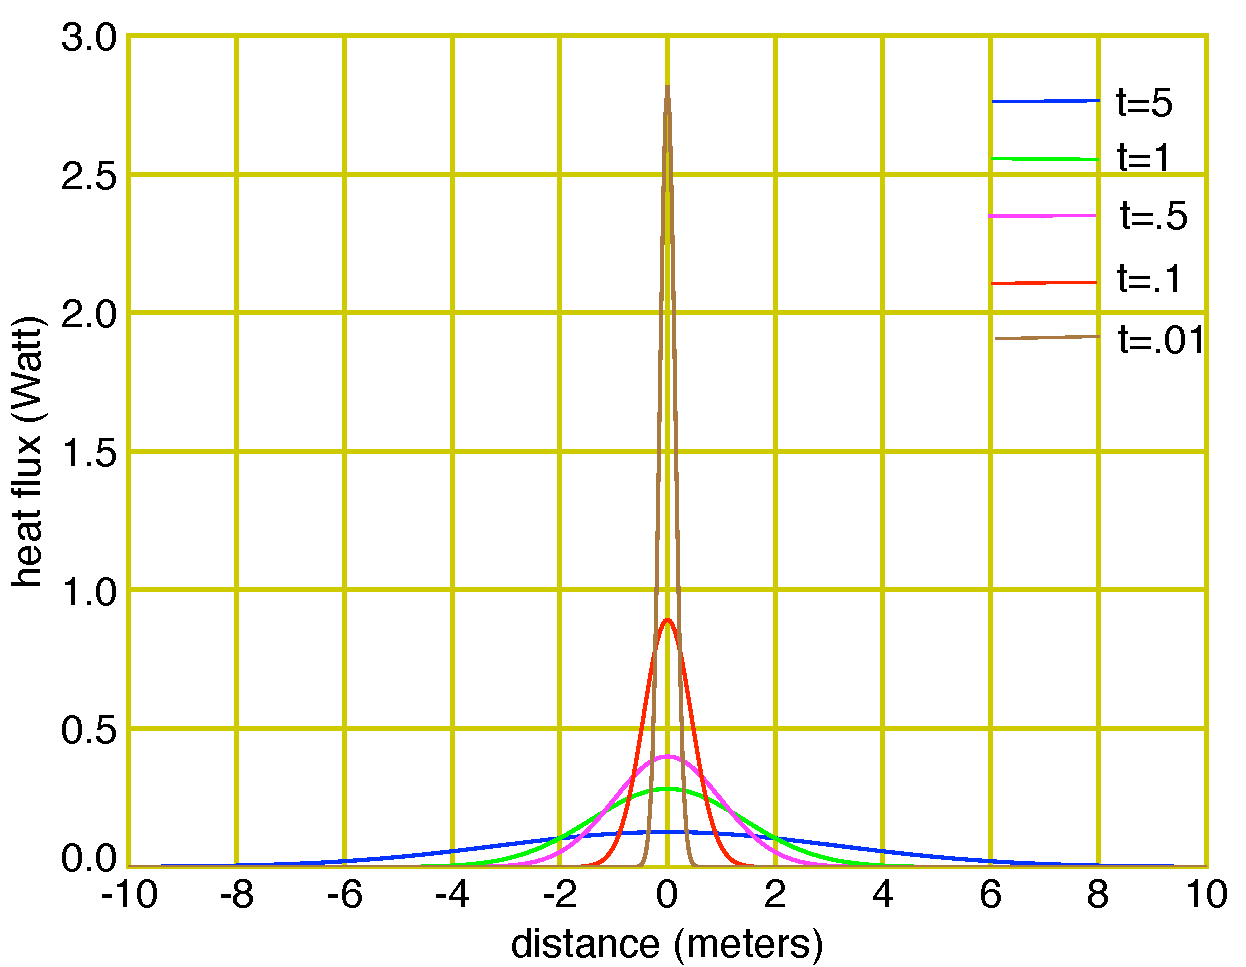
\includegraphics[width=1.\textwidth]{stufflinear.pdf}
\caption{Results of the {\tt heat.f95} code plotted on a linear scale. }
\label{linearscattering}
\end{figure}

\begin{figure}[!htb]
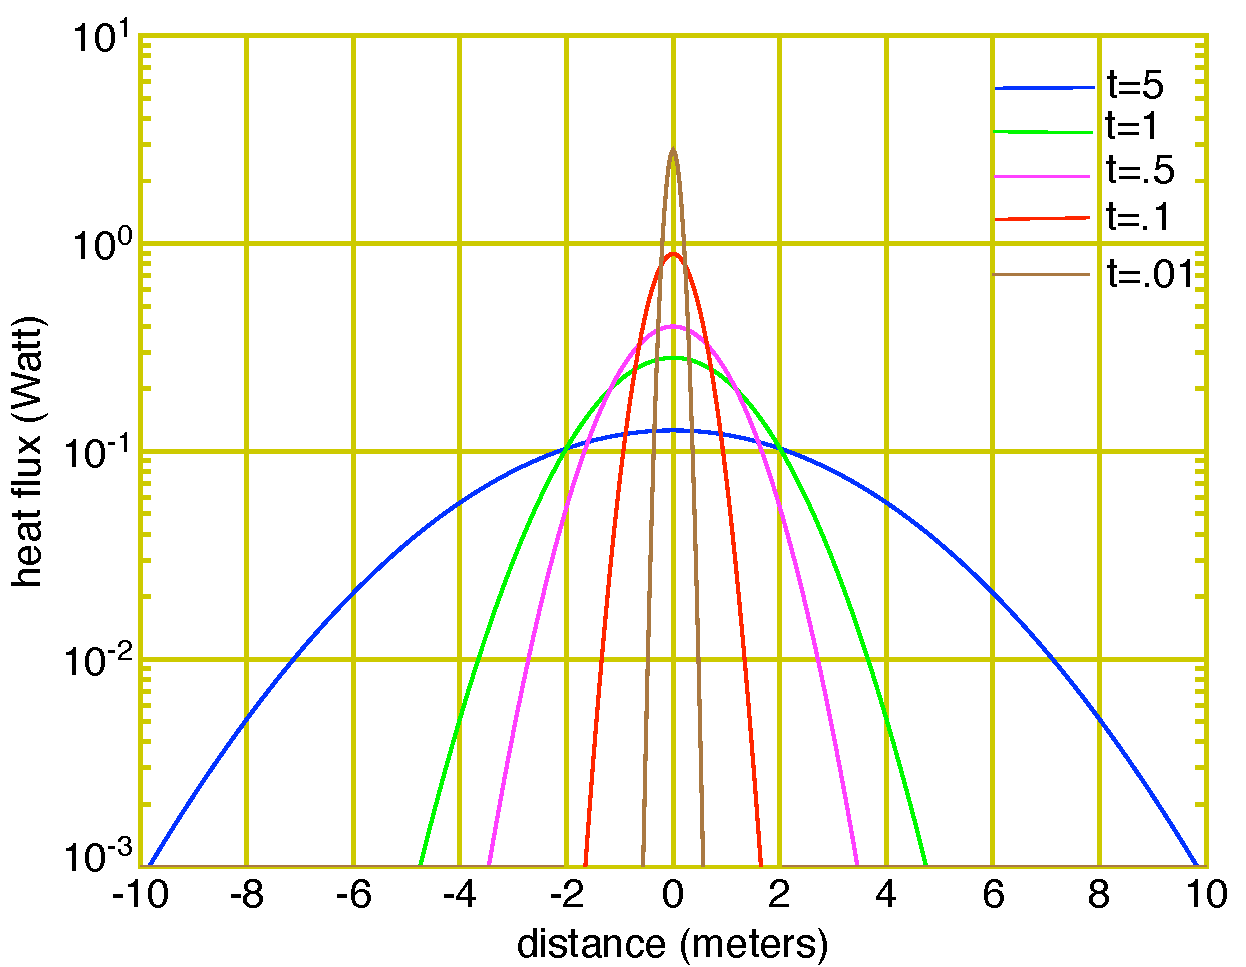
\includegraphics[width=1.\textwidth]{stufflog.pdf}
\caption{Results of the {\tt heat.f95} code plotted on a log scale. }
\label{logscattering}
\end{figure}





\section{Summary and conclusions}

The first Fortran95 code \cite{metcalf} for the class was written. The heat flux as a function of $\Theta$ with five different $t$ values were plotted. The graph demonstrates that as $t$ increases the data is more broadly distributed with a smaller maximum heat flux.

\begin{thebibliography}{}


\bibitem{metcalf} M.\ Metcalf, J.\ Reid and M.\ Cohen, {\it Fortran 95/2003 explained}. Oxford University Press, 2004.
 

\end{thebibliography}




\end{document}
